% !TEX TS-program = pdflatexmk
\documentclass[12pt]{article}
\usepackage{float}

\usepackage{amsthm}

% Layout.
\usepackage[top=.75in, bottom=0.75in, left=.75in, right=.75in, headheight=1in, headsep=6pt]{geometry}

\usepackage{fancyhdr, enumerate,multirow}
% Fonts.
\usepackage{mathptmx}
\usepackage[scaled=0.86]{helvet}
\renewcommand{\emph}[1]{\textsf{\textbf{#1}}}

% Misc packages.
\usepackage{amsmath,amssymb,latexsym}
\usepackage{graphicx,tikz}
\usepackage{array}
\usepackage{xcolor}
\usepackage{multicol}
\usepackage{tabularx,colortbl}
\usepackage[T1]{fontenc}
\usepackage{enumitem}
%to make tikz pics work
\usepackage{tikz,pgfplots}

\usepackage{varwidth}
\usepackage{verbatim}

\newenvironment{centerverbatim}{%
  \par
  \centering
  \varwidth{\linewidth}%
  \verbatim
}{%
  \endverbatim
  \endvarwidth
  \par
}

\makeatletter
\newenvironment{centeredverbatim}{\expandafter\verbatim\centering}{\endverbatim}
\makeatother


\usetikzlibrary{arrows}
\newcommand{\midarrow}{\tikz \draw[-triangle 90] (0,0) -- +(.1,0);}

\usepackage[colorlinks=true]{hyperref}

% Paragraph spacing
\parindent 0pt
\parskip 6pt plus 1pt
\def\tableindent{\hskip 0.5 in}
\def\ts{\hskip 1.5 em}

\usepackage{fancyhdr}
\pagestyle{fancy} 
\lhead{\large\sf\textbf{MATH 663 }}
\rhead{\large\sf\textbf{Fall 2023}}
\chead{\large\sf\textbf{HW 6}}

\newcommand{\localhead}[1]{\par\smallskip\textbf{#1}\nobreak\\}%
\def\heading#1{\localhead{\large\emph{#1}}}
\def\subheading#1{\localhead{\emph{#1}}}

%% Special Math Symbol shortcuts
\newcommand{\NN}{\mathbb{N}}
\newcommand{\RR}{\mathbb{R}}

\newcommand{\rad}{\text{rad}}
\newcommand{\diam}{\text{diam}}
\newcommand\solution{\localhead{Solution:}}

%\newenvironment{clist}%
%{\bgroup\parskip 0pt\begin{list}{$\bullet$}{\partopsep 4pt\topsep 0pt\itemsep -2pt}}%
%{\end{list}\egroup}%

\usetikzlibrary{calc,arrows.meta}
%\pgfplotsset{my style/.append style={axis x line=middle, axis y line=
%middle, xlabel={$x$}, ylabel={$y$}, axis equal }}{


\begin{document}
\begin{enumerate}
	\item Use Euler's Formula to prove that $K_{3,3}$ is not planar. 
	\begin{proof} Suppose for the sake of contradiction that $K_{3, 3}$ is planar. Let $G$ be a plane graph, embedding $K_{3, 3}$ and note that since $K_{3,3}$ is connected, so is $G$. By Euler's Formula it follows that, 
		\begin{equation*}
			6 - 9 + \ell = 2
		\end{equation*}
		Which implies that $G$ must have 5 faces. However since $K_{3, 3}$ is bipartite, there are no odd cycles, so each face in $G$ must contain at least 4 edges. Therefore the number of edges in $G$ is at least, 
		\begin{equation*}
			|E(G)| \geq \dfrac{(4)(5)}{2} = 10
		\end{equation*}
		Since the number of edges stays constant via an embedding and $|E(K_{3, 3})| = |E(G)| = 9$ we have a contradiction. 
	\end{proof}
	\newpage


	%Extra Credit
	\item Show that every connected planar graph with minimum degree at most 3 is a union of three forests.
	\begin{proof}
	\end{proof} 
	\newpage




	\item Show that every planar graph contains a vertex of degree at most 5. Give an example of a planar graph $G$ such that $\delta(G) \geq 5$
	\begin{proof} Suppose $G$ is a planar graph on $n$ vertices, and suppose for the sake of contradiction that for every $v \in G$, $d(v) \geq 6$. First note that $n \geq 3$ since any $2$ vertex simple graph cannot achieve $d(v) \geq 6$. Recall that,
		\begin{equation*}
			|E(G)| = \frac{1}{2} \sum_{v \in V(G)}d(v) \geq \frac{1}{2}(6n) = 3n
		\end{equation*}
		However, we have shown that a plane triangulation on $n \geq 3$ vertices has at most $3n - 6$ edges. Since plane triangulations are edge maximal plane graphs $G$ cannot be planar, since $|E(G)| \geq 3n > 3n - 6$. 
	\end{proof}

	\begin{figure}[H]
		\caption{Example of a planar $G$ with $\delta(G) \geq 5$.}
		\begin{center}
			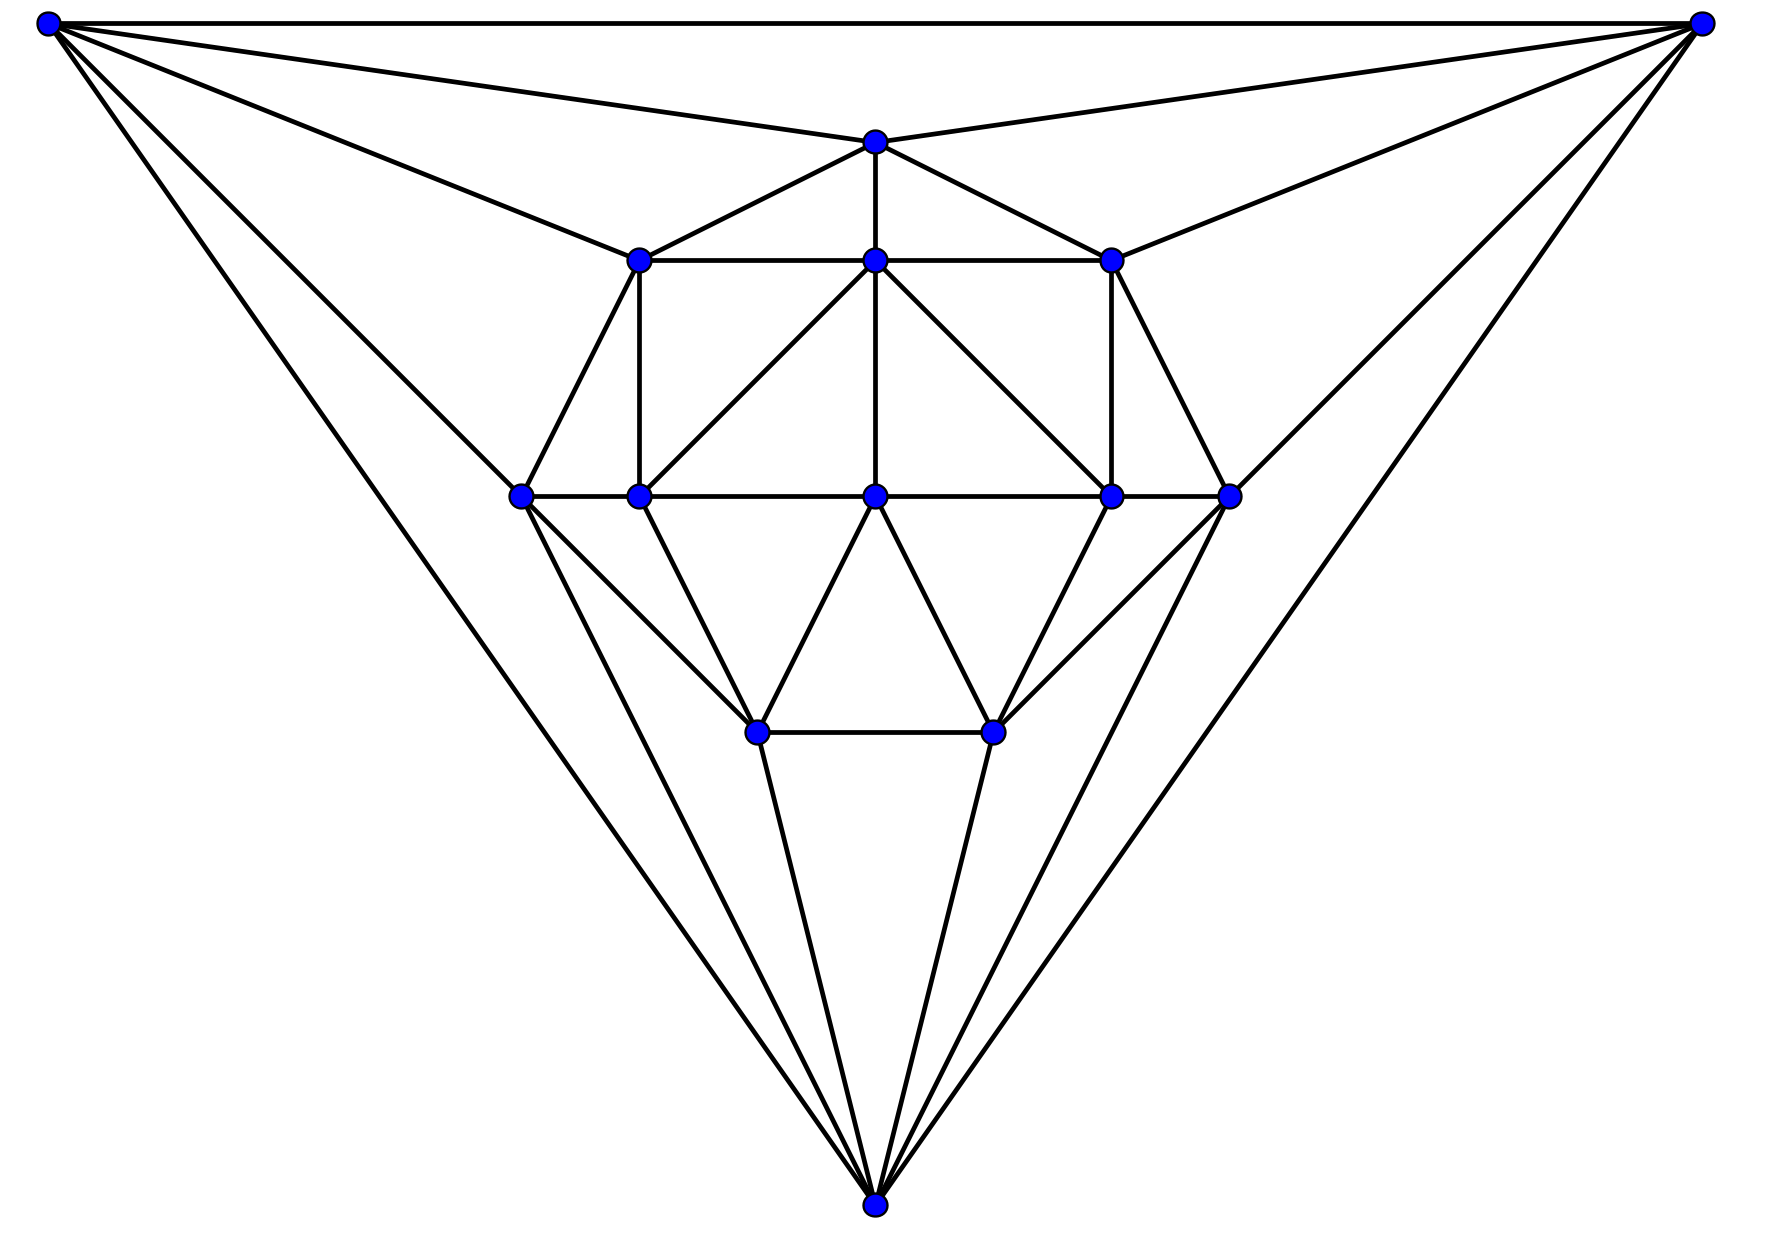
\includegraphics[width=.55\textwidth]{planargraphmin5.png}
		\end{center}
	\end{figure}
	\newpage




	\item A graph is called \emph{outerplanar} if it has a drawing in which every vertex lies on the boundary of the outer (or infinite) face. Show that a graph is outerplanar if and only if it does not contains a $K^4$ minor or a $K_{2, 3}$ minor.
	\begin{proof} $\rightarrow$ Suppose a graph $G$ is outerplanar and for the sake of contradiction suppose $G$ contains a $K_{2, 3}$ or $K_{4}$ minor. Let $\iota(G)$ be a plane graph via an embedding $\iota$. Note that adding a vertex to the interior of a face and arcs to all the vertices on the boundary of that face, maintains planarity. Therefore, since $G$ is outerplanar we can construct a plane graph $G' = \iota(G) + v$ where $v$ is a vertex on the interior of the infinite face, such that $v$ is incident to every vertex of $\iota(G)$. Since $G'$ is still a plane graph, Kuratowski's Thoerem applies and we find that $G'$ contains no $K_5$ or $K_{3, 3}$ minor. However clearly a $K_{2, 3}$ minor in $\iota(G)$ can be made into a $K_{3, 3}$ minor in $G'$ by adding $v$ to the partite set with 2 vertices, and clearly a $K_4$ minor in $\iota(G)$ can be made into a $K_5$ in $G'$ by considering $v$ as the fifth vertex. Thus a contradiction. 
	\end{proof}




		\begin{proof}$\leftarrow$ Suppose $G$ does not contain a $K^4$ minor or a $K_{2, 3}$ minor. Let $G' = G + v$ such that $v$ is a vertex incident to all vertices in $G$. Note $G'$ cannot have a $K_{3, 3}$ or $K_5$ minor, since any such minor would necessarily have to include vertex $v$, as $G$ has no $K^4$ minor or a $K_{2, 3}$ minor however, such a minor in $G'$ would imply the existence of a $K^4$ minor or a $K_{2, 3}$ minor in $G$. By Kuratowski's Theorem $G'$ is planar, furthermore there exists an embedding of $G'$, call it $\iota$, where $v$ is contained in the outer face of $G$ (this can be shown via a composition of homeomorphisms $\phi : \RR^2 \to S^{2,*}$ and $\rho : S^{2,*} \to S^{2,*}$ where $\rho$ moves the hole to the outer face of $G$). Now consider removing $v$ from $\iota(G')$, and since $v$ is contained in the outer face of $G$, $\iota(G') - v$ is now an outerplanar embedding of $G$.   
		
	\end{proof}
	\newpage
	
	









	\item Let $G$ be a 2-connected plane graph. Show $G$ is bipartite if and only if every face is bounded by an even cycle. 
	\begin{proof} $(\leftarrow)$ Let $G$ be a 2-connected plane graph, and suppose that every face is bounded by an even cycle. Suppose for the sake of contradiction that $G$ is not biparite. Then, $G$ contains an odd cycle call it $C$. Either $C$ bounds a face of $G$ and we've found a contradiction or, $C$ bounds multiple faces of $G$. Therefore there exists an arc of $G$ contained in $C$ which splits $C$  into an odd and even cycle. Proceeding iteratively there must exists an odd cycle bounding a face, a contradiction. 
 	\end{proof}

	\begin{proof}$(\rightarrow)$ Let $G$ be a 2-connected plane graph, and suppose $G$ is bipartite. Since $G$ is bipartite, it has no odd cycles, so all its cycles are even. Every face is bounded by a cycle which must necessarily be even. 
	\end{proof}
	\newpage











	\item Given a plane graph $G$, the \emph{dual graph} $G^*$, of $G$ is a plane graph whose vertices correspond to the faces of $G$. The edges of $G^*$ are defined as follows: for every edge $e \in E(G)$ on the boundary of faces $X$ and $Y$ in $G$, edge $\{X, Y\} \in E(G^*)$. Note that the dual graph of a simple plane graph may or may not be simple. 
	\begin{enumerate}
		\item[(a)] Describe the dual graphs of $P^m$, $C^k$, and $K^4$. 
		\solution
		The dual graph of $P^m$ looks like a single vertex with $m - 1$ loops, since each edge of $P^m$ bounds the infinite face twice.\\

		The dual graph of $C^k$ is a pair of vertices, one representing the enclosed face, and the other representing the infinite face with $k$ arcs in between. \\

		The dual graph of $K^4$ is another $K^4$. \\

		





		\item[(b)] Prove that if the $n$-vertex plane graph $G$ is isomorphic to its dual, $G^*$, then $\lvert|G|\rvert = 2n - 2$.  
		\begin{proof} Suppose that $G$ is an $n$-vertex plane graph, which is isomorphic to it's dual $G^*$. By the construction of $G^*$ the number of faces of $G$ and is equal to the vertices of $G^*$, since $G$ and $G^*$ are isomorphic, they have the same number of vertices, and therefore, $G$ has the same number of vertices and faces. Applying Euler's Formula to $G$ with $n = f$ we find that, 
			\begin{align*}
				n - e + f &= 2,\\
				n - e + n &= 2,\\
				2n - 2&=e.
			\end{align*}
		\end{proof}
	\end{enumerate}


	
	
	
	

















\end{enumerate}
\end{document}


